\begin{pastexam}[label={px:ccu-113-swa-02}]{中正資工所甲組 113 學年度 第 2 題}
（單選）

The following is an AVL tree, which is implemented/represented as an array. Please answer the following questions from Q1 to Q3.

\begin{center}
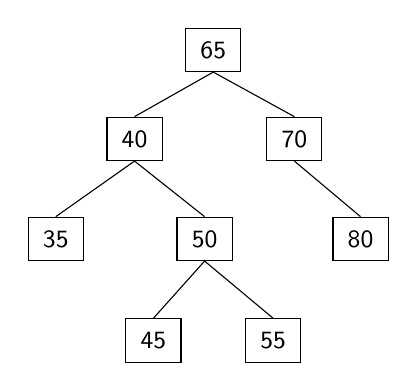
\begin{tikzpicture}[font=\sffamily\small]
\node[draw,rectangle,minimum width=7mm,minimum height=5.5mm,inner sep=1pt] (a) at (7.08,-5.92) {65};
\node[draw,rectangle,minimum width=7mm,minimum height=5.5mm,inner sep=1pt] (b) at (6.08,-7.05) {40};
\node[draw,rectangle,minimum width=7mm,minimum height=5.5mm,inner sep=1pt] (c) at (8.11,-7.05) {70};
\node[draw,rectangle,minimum width=7mm,minimum height=5.5mm,inner sep=1pt] (d) at (5.08,-8.32) {35};
\node[draw,rectangle,minimum width=7mm,minimum height=5.5mm,inner sep=1pt] (e) at (6.97,-8.32) {50};
\node[draw,rectangle,minimum width=7mm,minimum height=5.5mm,inner sep=1pt] (f) at (8.95,-8.32) {80};
\node[draw,rectangle,minimum width=7mm,minimum height=5.5mm,inner sep=1pt] (g) at (6.32,-9.61) {45};
\node[draw,rectangle,minimum width=7mm,minimum height=5.5mm,inner sep=1pt] (h) at (7.84,-9.61) {55};
\draw (a.south)--(b.north) (a.south)--(c.north) (b.south)--(d.north) (b.south)--(e.north) (c.south)--(f.north) (e.south)--(g.north) (e.south)--(h.north);
\end{tikzpicture}
\end{center}

(3\%) Perform the post-order traversal on the AVL tree constructed for the first question (Q1) after the insertion. What is the sequence of nodes in the post-order traversal of the AVL tree?
\begin{enumerate}[label=\Alph*.]
\item 35$\to$43$\to$45$\to$55$\to$50$\to$40$\to$80$\to$70$\to$65
\item 35$\to$43$\to$55$\to$50$\to$45$\to$40$\to$80$\to$70$\to$65
\item 35$\to$43$\to$40$\to$55$\to$50$\to$45$\to$80$\to$70$\to$65
\item 65$\to$40$\to$35$\to$50$\to$45$\to$43$\to$55$\to$70$\to$80
\item None of the above
\end{enumerate}
\end{pastexam}

\begin{pastsoln}
答案是 C。

第 1 題插入 $43$ 之後的樹（見歷屆試題~\ref{px:ccu-113-swa-01}）是
\[
65\Bigl(45\bigl(40(35, 43),\ 50(-, 55)\bigr),\ 70(-, 80)\Bigr).
\]
後序是「左子樹、右子樹、根」（資結書第~7.3~節）：
\begin{itemize}
\item $40$ 的子樹：$35, 43, 40$。
\item $50$ 的子樹：左邊空，$55, 50$。
\item $45$ 的子樹：$35, 43, 40, 55, 50, 45$。
\item $70$ 的子樹：$80, 70$。
\item 最後是根 $65$。
\end{itemize}
得 $35 \to 43 \to 40 \to 55 \to 50 \to 45 \to 80 \to 70 \to 65$，就是 C。

逐項檢查：
\begin{itemize}
\item A：$35, 43, 45, 55, 50, 40, \ldots$ 是插入時\textbf{沒有旋轉}的樹 $40(35, 50(45(43, -), 55))$ 的後序。 錯。
\item B：$40$ 排在 $45$ 後面、$55, 50$ 前面也不對；$40$ 的子樹走完就要輸出 $40$。 錯。
\item C：上面的結果。 對。
\item D：第一個是 $65$，這是前序的寫法（根先），不是後序。 錯。
\item E：C 是對的。 錯。
\end{itemize}
\end{pastsoln}
